\subsection{Question 1}

\subsubsection{Vandermonde}

\begin{equation}
	\begin{aligned}
		\begin{pmatrix}
			1 & 12 & 144\\
			1 & 20 & 400\\
			1 & 24 & 576
		\end{pmatrix}
		\cdot
		\begin{pmatrix}
			a_1\\
			a_2\\
			a_3
		\end{pmatrix}=
		\begin{pmatrix}
			4\\
			16\\
			17
		\end{pmatrix}
	\end{aligned}
\end{equation}

On peut ensuite trouver les valeurs $a_1$, $a_2$ et $a_3$ en résolvant le système.

Ici, nous n'avons pas fait ce développement, nous avons simplement entré la matrice dans la méthode de résolution par Gauss-Jordan implémentée dans la première question de la leçon 3.

Nous obtenons ainsi :

\begin{equation}
	\begin{aligned}
		a_1 &= -39\\
		a_2 &= 4.833\\
		a_3 &= -0.104
	\end{aligned}
\end{equation}

\subsubsection{Lagrange}

\begin{equation}
	f(x) = (y^{(1)} \cdot \Phi_1(x)) + (y^{(2)} \cdot \Phi_2(x)) + (y^{(3)} \cdot \Phi_3(x))
\end{equation}

\begin{equation}
	\begin{aligned}
		\Phi_1(x) &= \frac{(x-x^{(2)})(x-x^{(3)})}{(x^{(1)}-x^{(2)})(x^{(1)}-x^{(3)})} = \frac{(x-20)(x-24)}{96} = \frac{x^2}{96} - \frac{11}{24}x+5\\
		\Phi_1(x) &= \frac{(x-x^{(1)})(x-x^{(3)})}{(x^{(2)}-x^{(1)})(x^{(2)}-x^{(3)})} = \frac{(x-12)(x-24)}{-32} = \frac{-3x^2}{96} + \frac{27}{24}x - 9\\
		\Phi_1(x) &= \frac{(x-x^{(1)})(x-x^{(2)})}{(x^{(3)}-x^{(1)})(x^{(3)}-x^{(2)})} = \frac{(x-12)(x-20)}{48} = \frac{2x^2}{96} - \frac{16}{24}x + 5
	\end{aligned}
\end{equation}


\begin{equation}
	\begin{aligned}
		f(x) = \frac{-5}{48}x^2 + \frac{29}{6}x-144
	\end{aligned}
\end{equation}

\subsubsection{Newton}

\begin{equation}
	\begin{aligned}
		\Psi_1(x) &= 1\\
		\Psi_2(x) &= \Psi_1(x) \cdot (x-12)\\
		\Psi_3(x) &= \Psi_2(x) \cdot (x-20) = (x-12)(x-20)\\
	\end{aligned}
\end{equation}

\begin{equation}
	\begin{pmatrix}
		1 & 0 & 0\\
		1 & 8 & 0\\
		1 & 12 & 48
	\end{pmatrix}\cdot
	\begin{pmatrix}
		c_1\\
		c_2\\
		c_3
	\end{pmatrix}=
	\begin{pmatrix}
		4\\
		16\\
		17
	\end{pmatrix}
\end{equation}

A l'aide de notre méthode Java pour Gauss-Jordan, nous obtenons que 

\begin{equation}
	\begin{aligned}
		c_1 &= 4\\
		c_2 &= 1.5\\
		c_3 &= -0.104
	\end{aligned}
\end{equation}

Nous pouvons alors définir $f(x)$ :

\begin{equation}
	f(x) = 4 + 1.5(x-12) - 0.104(x-12)(x-20)
\end{equation}


\begin{figure}[H]
\caption{\label{3pts} Interpolation avec 3 points}
\centering
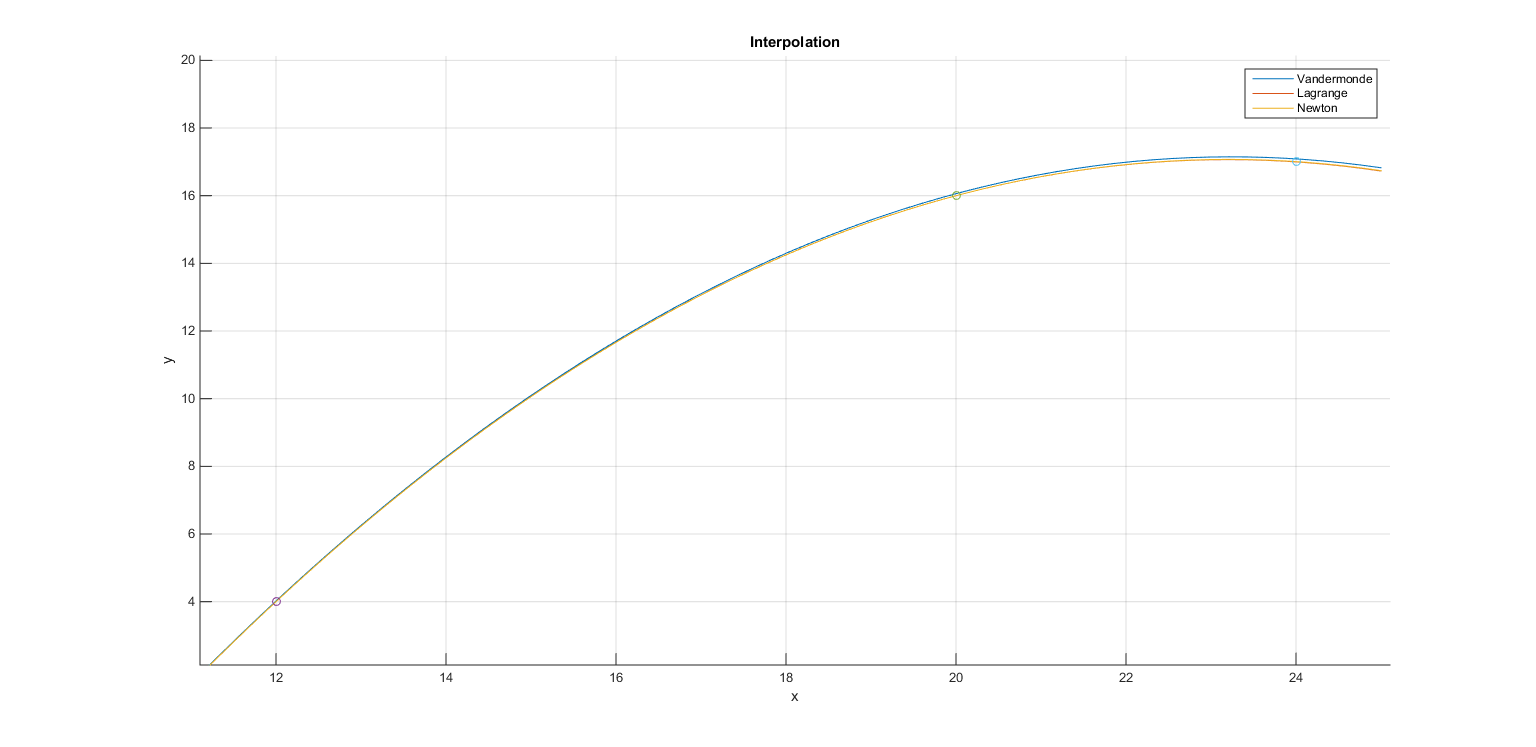
\includegraphics[scale = 0.4]{Figures/6_interpolation.png}
\end{figure}

\subsubsection{Vandermonde avec une mesure en plus}

\begin{equation}
	\begin{aligned}
		\begin{pmatrix}
			1 & 12 & 144 & 1728\\
			1 & 20 & 400 & 8000\\
			1 & 24 & 576 & 13824\\
			1 & 16 & 256 & 4096
		\end{pmatrix}
		\cdot
		\begin{pmatrix}
			a_1\\
			a_2\\
			a_3\\
			a_4
		\end{pmatrix}
		=
		\begin{pmatrix}
			4\\
			16\\
			17\\
			13
		\end{pmatrix}
	\end{aligned}
\end{equation}

On peut ensuite trouver les valeurs $a_1$, $a_2$, $a_3$ et $a_4$ en résolvant le système. Nous obtenons ainsi :

\begin{equation}
	\begin{aligned}
		a_1 &= -99\\
		a_2 &= 46/3\\
		a_3 &= -11/16\\
		a_4 &= 1/96
	\end{aligned}
\end{equation}

\subsubsection{Newton avec une mesure en plus}

\begin{equation}
	\begin{aligned}
		f(x) &= 4 + 1.5(x-12) - 0.104(x-12)(x-20) + c_4(x-12)(x-20)(x-24)\\
		f(16) &= 13\\
		13 &= 10 + \frac{80}{48}+128c_4\\
		c_4 &= \frac{3-80/48}{128} = \frac{1}{96}
	\end{aligned}
\end{equation}

\begin{figure}[H]
	\centering
	\caption{\label{4pts} Interpolation avec 4 points}
	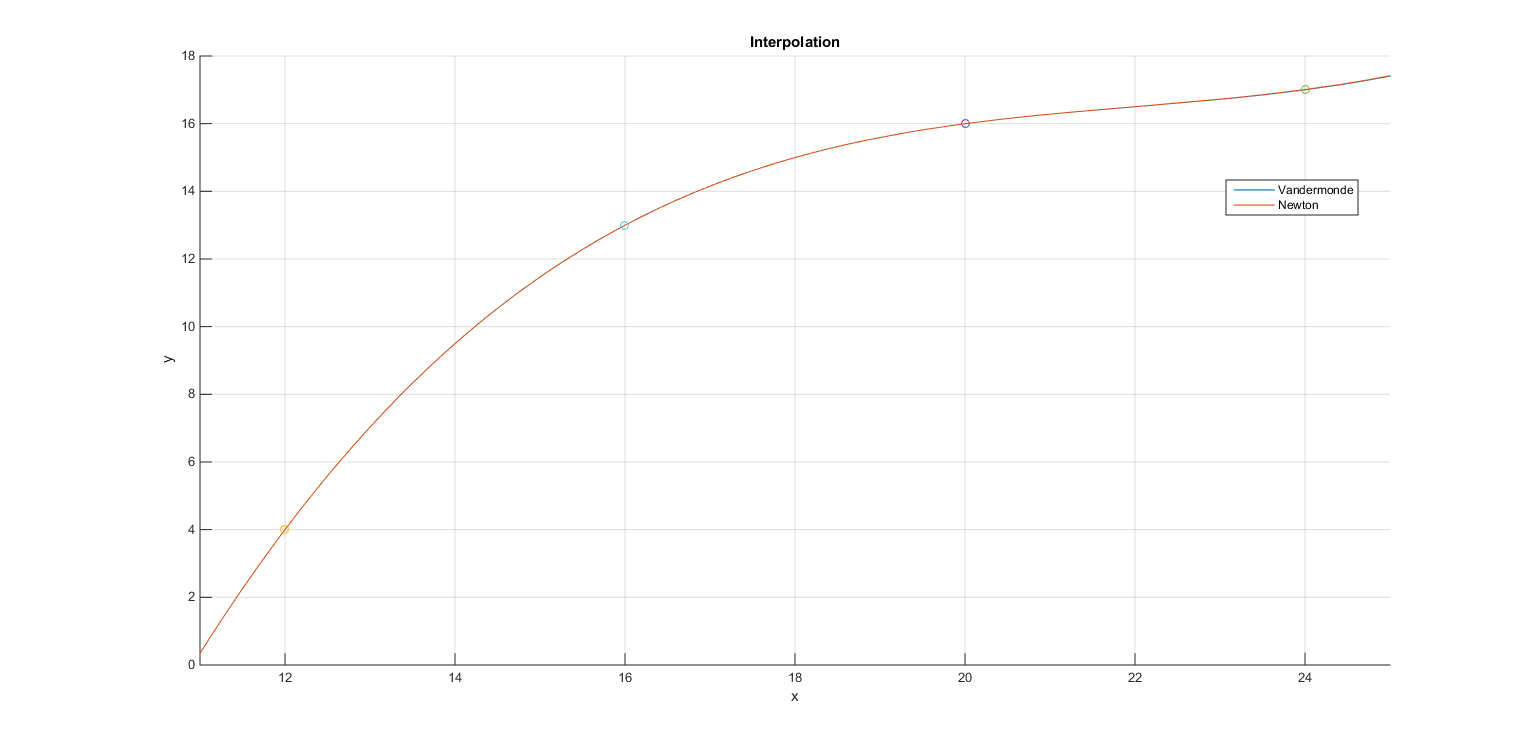
\includegraphics[scale = 0.4]{Figures/6_interpolation_2.png}
\end{figure}

\begin{figure}[H]
	\centering
	\caption{\label{3ou4} Interpolation via Newton avec 3 ou 4 points}
	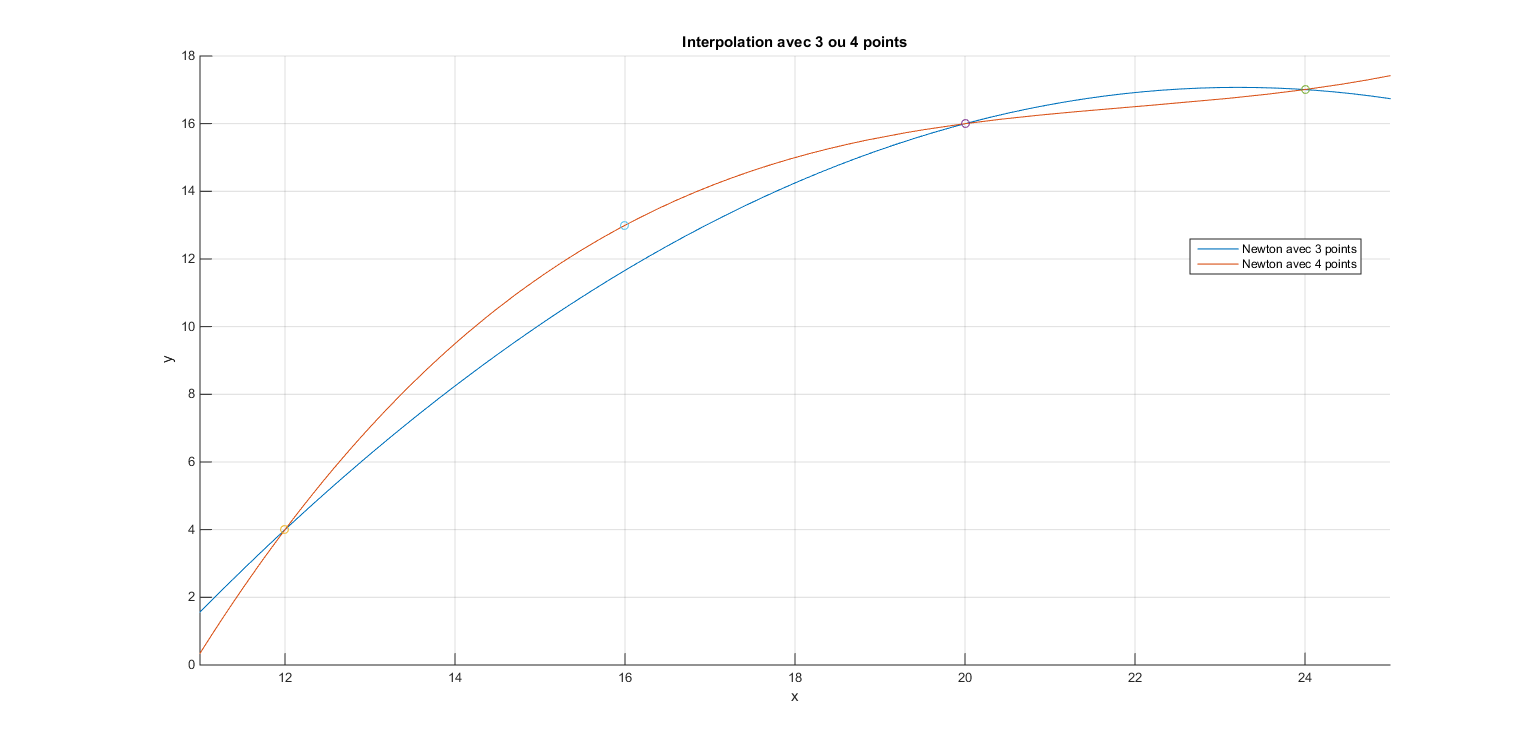
\includegraphics[scale = 0.4]{Figures/6_interpolation_3ou4.png}
\end{figure}


\subsection{Question 2}

Tous les codes de cette question sont dans le projet \texttt{numalgoplotter} qui est basé sur les codes fournis sur moodle. 

\subsubsection{NumAlgoPlotter}
\code{numalgoplotter}{NumAlgoPlotter.java}

\subsubsection{VandermondePlotter}
\code{numalgoplotter}{VandermondePlotter.java}

\begin{figure}[H]
	\centering
	\caption{\label{vandermonde} VandermondePlotter}
	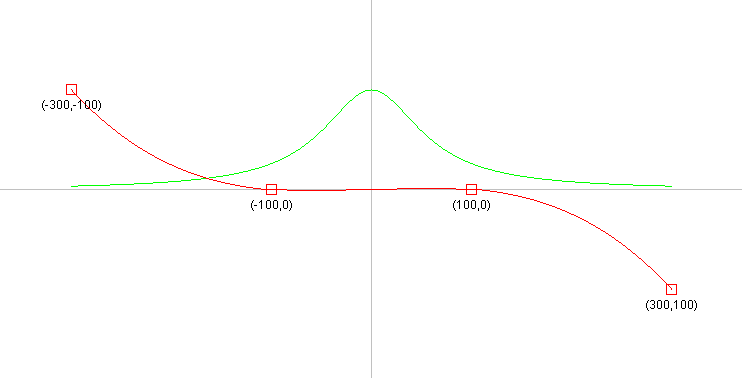
\includegraphics[scale = 0.4]{Figures/6_VandermondePlotter.png}
\end{figure}

\subsubsection{NewtonPlotter}
\code{numalgoplotter}{NewtonPlotter.java}

\begin{figure}[H]
	\centering
	\caption{\label{newton} NewtonPlotter}
	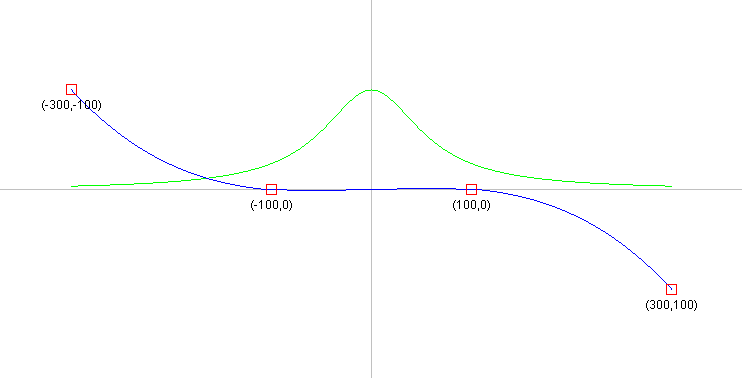
\includegraphics[scale = 0.4]{Figures/6_NewtonPlotter.png}
\end{figure}